\documentclass[aspectratio=169,10pt]{beamer}

\usetheme{default}
\usecolortheme{default}
\usefonttheme{professionalfonts}
\usepackage{tikz}
\usepackage{amsmath}
\usetikzlibrary{positioning}

\definecolor{aggieMaroon}{HTML}{500000}
\definecolor{aggieDarkMaroon}{HTML}{3C0000}
\definecolor{aggieGray}{HTML}{707373}
\definecolor{aggieLightGray}{HTML}{F2F2F2}

\setbeamercolor{normal text}{fg=black,bg=white}
\setbeamercolor{structure}{fg=aggieMaroon}
\setbeamercolor{frametitle}{fg=white,bg=aggieMaroon}
\setbeamercolor{title}{fg=white}
\setbeamercolor{subtitle}{fg=white}
\setbeamercolor{author}{fg=white}
\setbeamercolor{institute}{fg=white}
\setbeamercolor{date}{fg=white}
\setbeamercolor{block title}{fg=white,bg=aggieMaroon}
\setbeamercolor{block body}{fg=black,bg=aggieLightGray}
\setbeamercolor{itemize item}{fg=aggieMaroon}
\setbeamercolor{itemize subitem}{fg=aggieMaroon}

\setbeamertemplate{navigation symbols}{}
\setbeamertemplate{items}[circle]
\setbeamertemplate{frametitle}{%
  \nointerlineskip
  \begin{beamercolorbox}[wd=\paperwidth,ht=0.82cm,dp=0.22cm,leftskip=0.65cm]{frametitle}%
    \usebeamerfont{frametitle}\insertframetitle
  \end{beamercolorbox}%
}

\title{Options Pricing}
\subtitle{Replication, no-arbitrage, and the binomial model}
\author{}
\institute{}
\date{\today}

\begin{document}

\begin{frame}{What Is an Option?}
  \begin{columns}[T,onlytextwidth]
    \begin{column}{0.58\textwidth}
      \textbf{An option} gives its holder the \alert{right, not the obligation}, to transact in an underlying asset on specified terms.
      \vspace{0.35cm}
      \begin{itemize}
        \item \textbf{Call:} right to buy at the strike price $K$.
        \item \textbf{Put:} right to sell at the strike price $K$.
        \item \textbf{Expiration $T$:} last date the right can be exercised.
        \item \textbf{Premium:} price paid today for the contract.
      \end{itemize}
    \end{column}
    \begin{column}{0.38\textwidth}
      \begin{block}{Central question}
        How much should someone pay today for a claim that provides a potentially uncertain payoff in the future?
      \end{block}
    \end{column}
  \end{columns}
\end{frame}

\begin{frame}{An Arbitrary Financial Claim}
  \begin{columns}[c,onlytextwidth]
    \begin{column}{0.48\textwidth}
      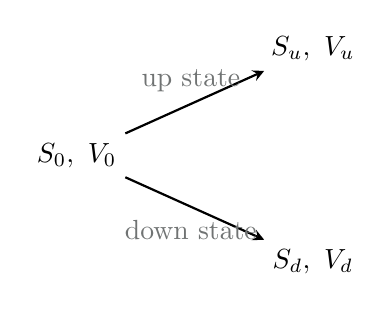
\begin{tikzpicture}[x=1cm,y=1cm,>=stealth]
        \node (zero) at (0,0) {$S_0,\ V_0$};
        \node (up) at (3,1.35) {$S_u,\ V_u$};
        \node (down) at (3,-1.35) {$S_d,\ V_d$};
        \draw[->,thick] (zero) -- (up);
        \draw[->,thick] (zero) -- (down);
        \node[aggieGray] at (1.45,0.95) {up state};
        \node[aggieGray] at (1.45,-0.95) {down state};
      \end{tikzpicture}
    \end{column}
    \begin{column}{0.48\textwidth}
      Suppose a stock trades today at $S_0$. At time $T$, it can be $S_u$ or $S_d$.
      \vspace{0.25cm}
      A claim $V$ written on the stock then pays $V_u$ or $V_d$.
    \end{column}
  \end{columns}
\end{frame}

\begin{frame}{Replicating the Financial Claim}
  Rather than price the claim directly, build a portfolio with exactly the same payoff in every state.
  \vspace{0.3cm}
  \begin{columns}[T,onlytextwidth]
    \begin{column}{0.47\textwidth}
      Hold $\Delta$ shares of stock and borrow $y$ dollars today at continuously compounded rate $r$.
      \vspace{0.2cm}
      \small
      $\Delta$ is the shares you have bought; $y$ is the amount of the loan.
    \end{column}
    \begin{column}{0.48\textwidth}
      \begin{align*}
        V_u &= \Delta S_u - y e^{rT},\\
        V_d &= \Delta S_d - y e^{rT}.
      \end{align*}
    \end{column}
  \end{columns}
\end{frame}

\begin{frame}{Solving for $\Delta$ and the Loan}
  \begin{align*}
    V_u - V_d &= \Delta(S_u-S_d) \\[0.15cm]
    \therefore\qquad \Delta &= \frac{V_u-V_d}{S_u-S_d}\\[0.15cm]
    y &= e^{-rT}(\Delta S_d-V_d)
  \end{align*}
  \begin{center}
    $\Delta$ is the shares you have bought. \hspace{1cm} $y$ is the amount of the loan.
  \end{center}
\end{frame}

\begin{frame}{No-Arbitrage: The Law of One Price}
  \begin{block}{Portfolio lemma}
    If two portfolios have identical future payoffs in every state, then an arbitrage-free market must assign them the same price today.
  \end{block}
  \vspace{0.25cm}
  \begin{center}
    \Large $\displaystyle V_0 = \Delta S_0-y$
  \end{center}
\end{frame}

\begin{frame}{A One-Step Call Option Example}
  \small
  $S_0=\$100$, $S_u=\$120$, $S_d=\$80$, $K=\$100$, and $r=0$. Therefore,
  \begin{align*}
    V_u&=\max(120-100,0)=\$20, & V_d&=\max(80-100,0)=\$0,\\
    \Delta&=\frac{20-0}{120-80}=0.5, & y&=0.5(80)-0=\$40,\\
    V_0&=0.5(100)-40=\boxed{\$10}.
  \end{align*}
  \begin{columns}[T,onlytextwidth]
    \begin{column}{0.47\textwidth}
      \begin{block}{Up state}
        Half a share is worth $\$60$. Repay $\$40$. Remaining payoff: $\$20$.
      \end{block}
    \end{column}
    \begin{column}{0.47\textwidth}
      \begin{block}{Down state}
        Half a share is worth $\$40$. Repay $\$40$. Remaining payoff: $\$0$.
      \end{block}
    \end{column}
  \end{columns}
  \vspace{0.1cm}
  \centering\textbf{The $\$10$ premium is paid today; $\$20$ or $\$0$ is paid at expiration.}
\end{frame}

\begin{frame}{From Replication to Risk-Neutral Pricing}
  Insert the replicating portfolio into $V_0=\Delta S_0-y$:
  \begin{align*}
    V_0 &= \Delta S_0-e^{-rT}(\Delta S_d-V_d)\\
        &= e^{-rT}\left[qV_u+(1-q)V_d\right],
  \end{align*}
  where
  \begin{center}
    \Large $\displaystyle q=\frac{S_0e^{rT}-S_d}{S_u-S_d}$.
  \end{center}
  \vspace{0.3cm}
  Interpretation:
\end{frame}

\begin{frame}{What Are Risk-Neutral Probabilities?}
  \begin{center}
    \Large $\displaystyle S_0=e^{-rT}\left[qS_u+(1-q)S_d\right]$
  \end{center}
  The weights $q$ and $1-q$ make the stock's expected return equal to the risk-free rate.
  \vspace{0.25cm}
  \begin{columns}[T,onlytextwidth]
    \begin{column}{0.47\textwidth}
      \begin{block}{Actual probabilities}
        Describe beliefs about what will happen in the world.
      \end{block}
    \end{column}
    \begin{column}{0.47\textwidth}
      \begin{block}{Risk-neutral probabilities}
        Are pricing weights consistent with traded-asset prices and no-arbitrage.
      \end{block}
    \end{column}
  \end{columns}
  \vspace{0.2cm}
  \begin{block}{No-arbitrage condition}
    $S_d<S_0e^{rT}<S_u$ ensures $0<q<1$. These weights arise from replication, not from forecasting the next stock move.
  \end{block}
\end{frame}

\begin{frame}{Extending to Multiple Time Steps}
  \begin{columns}[c,onlytextwidth]
    \begin{column}{0.50\textwidth}
      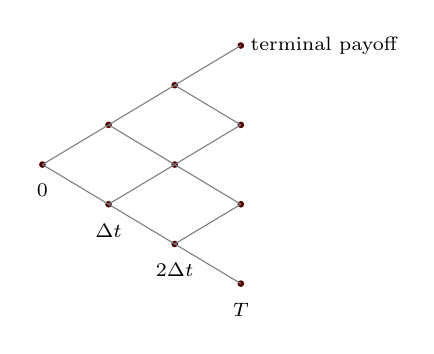
\begin{tikzpicture}[x=1.05cm,y=0.63cm,>=stealth,scale=0.8,every node/.style={font=\scriptsize}]
        \foreach \x/\y in {0/0,1/1,1/-1,2/2,2/0,2/-2,3/3,3/1,3/-1,3/-3}
          \fill[aggieMaroon] (\x,\y) circle (1.5pt);
        \foreach \a/\b/\c/\d in {0/0/1/1,0/0/1/-1,1/1/2/2,1/1/2/0,1/-1/2/0,1/-1/2/-2,2/2/3/3,2/2/3/1,2/0/3/1,2/0/3/-1,2/-2/3/-1,2/-2/3/-3}
          \draw[gray] (\a,\b)--(\c,\d);
        \node[below] at (0,-0.25) {$0$};
        \node[below] at (1,-1.25) {$\Delta t$};
        \node[below] at (2,-2.25) {$2\Delta t$};
        \node[below] at (3,-3.25) {$T$};
        \node[right] at (3,3) {terminal payoff};
      \end{tikzpicture}
    \end{column}
    \begin{column}{0.46\textwidth}
      At every terminal node, the contract tells us the payoff. Then work backward:
      \begin{align*}
        V_t=e^{-r\Delta t}\big[qV_{t+\Delta t}^{u}+(1-q)V_{t+\Delta t}^{d}\big].
      \end{align*}
      \small
      \begin{enumerate}
        \item Calculate terminal payoffs.
        \item Weight and discount adjacent values.
        \item Repeat until time zero.
      \end{enumerate}
    \end{column}
  \end{columns}
  \centering\small Terminal nodes are model-generated scenarios, not forecasts of realized prices.
\end{frame}

\begin{frame}{From Binomial Trees to Black--Scholes}
  \begin{columns}[T,onlytextwidth]
    \begin{column}{0.45\textwidth}
      \begin{block}{Discrete binomial model}
        Stock prices move up or down at individual time steps.
      \end{block}
      \centering\Large More steps, smaller $\Delta t$
    \end{column}
    \begin{column}{0.08\textwidth}
      \vspace{0.7cm}\centering\Large $\rightarrow$
    \end{column}
    \begin{column}{0.45\textwidth}
      \begin{block}{Continuous-time model}
        Stock prices evolve continuously under a stochastic process.
      \end{block}
    \end{column}
  \end{columns}
  \vspace{0.35cm}
  Under an appropriate parameterization, the binomial price converges to the Black--Scholes--Merton price as the number of steps grows.
\end{frame}

\begin{frame}{Black--Scholes--Merton: Equation and Price}
  \small
  Continuous-time delta hedging and no-arbitrage lead to
  \begin{align*}
    \frac{\partial V}{\partial t}+\frac{1}{2}\sigma^2S^2\frac{\partial^2V}{\partial S^2}+rS\frac{\partial V}{\partial S}-rV=0.
  \end{align*}
  \begin{columns}[T,onlytextwidth]
    \begin{column}{0.52\textwidth}
      For a European call with no dividends,
      \begin{align*}
        C&=S_0N(d_1)-Ke^{-rT}N(d_2),\\
        d_1&=\frac{\ln(S_0/K)+(r+\sigma^2/2)T}{\sigma\sqrt{T}},\quad d_2=d_1-\sigma\sqrt{T}.
      \end{align*}
    \end{column}
  \end{columns}
\end{frame}

\begin{frame}{The Greeks: Sensitivities of Option Value}
  \small
  \begin{columns}[T,onlytextwidth]
    \begin{column}{0.48\textwidth}
      \begin{block}{Delta: $\frac{\partial V}{\partial S}$}
        Sensitivity to stock price; locally, the shares needed to hedge the option.
      \end{block}
      \begin{block}{Gamma: $\frac{\partial^2 V}{\partial S^2}$}
        Sensitivity of Delta to the stock price.
      \end{block}
      \begin{block}{Theta}
        Sensitivity to time; its sign depends on whether time is calendar time or time to expiration.
      \end{block}
    \end{column}
    \begin{column}{0.48\textwidth}
      \begin{block}{Vega: $\frac{\partial V}{\partial \sigma}$}
        Sensitivity to volatility.
      \end{block}
      \begin{block}{Rho: $\frac{\partial V}{\partial r}$}
        Sensitivity to the interest rate.
      \end{block}
      \vspace{0.25cm}
      \textbf{Connection:} the $\Delta$ from the one-step replicating portfolio becomes a local, continuously adjusted hedge ratio.
    \end{column}
  \end{columns}
\end{frame}

\begin{frame}{Final Takeaway}
  \centering
  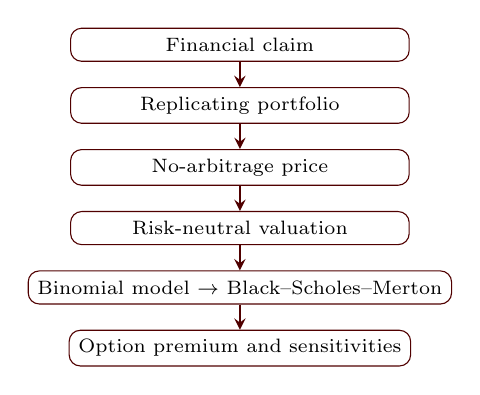
\begin{tikzpicture}[node distance=0.32cm,>=stealth,every node/.style={font=\scriptsize,align=center}]
    \node (a) [draw=aggieMaroon,rounded corners,minimum width=4.3cm,minimum height=0.42cm] {Financial claim};
    \node (b) [below=of a,draw=aggieMaroon,rounded corners,minimum width=4.3cm,minimum height=0.42cm] {Replicating portfolio};
    \node (c) [below=of b,draw=aggieMaroon,rounded corners,minimum width=4.3cm,minimum height=0.42cm] {No-arbitrage price};
    \node (d) [below=of c,draw=aggieMaroon,rounded corners,minimum width=4.3cm,minimum height=0.42cm] {Risk-neutral valuation};
    \node (e) [below=of d,draw=aggieMaroon,rounded corners,minimum width=4.3cm,minimum height=0.42cm] {Binomial model $\rightarrow$ Black--Scholes--Merton};
    \node (f) [below=of e,draw=aggieMaroon,rounded corners,minimum width=4.3cm,minimum height=0.42cm] {Option premium and sensitivities};
    \foreach \x/\y in {a/b,b/c,c/d,d/e,e/f} \draw[->,aggieMaroon,thick] (\x)--(\y);
  \end{tikzpicture}
  \vspace{0.1cm}
  \begin{block}{Central message}
    Options pricing is not fundamentally about predicting where a stock will go. It is about determining what a financial claim should cost today, given its possible future payoffs and the prices of tradable assets.
  \end{block}
\end{frame}

\end{document}
